\section{Explicit tower over the \texorpdfstring{$165$}{165}-measurement graph}\label{app:finite}

This appendix constructs the tower of length one over $F_{\rm phys}$ used in the proof of Theorem~\ref{thm:finite-square} (Section~\ref{sec:165}). Throughout, homology is taken with coefficients in $\Ftwo$, and we write $\mathbb T=\R/3\mathbb Z$ for the circle of circumference $3$ (so that $3$-coloring labels live naturally in $\mathbb Z/3\subset\mathbb T$).

\emph{Difference subcomplex $\Delta$ and the $21$-triangle filling.} Recall from~\eqref{eq:finite-words} the thirteen difference triples $p\in\{O,\alpha_i,\beta_i,\delta_i,\upsilon_i:i\in\mathbb Z/3\}$ in $(\mathbb Z/3)^3\subset\mathbb T^3$. Table~\ref{tab:triples} lists them together with the words that they give.

\begin{table}[htbp]
\centering
\small
\begin{tabular}{@{}l>{\raggedright\arraybackslash}p{3.5cm}>{\raggedright\arraybackslash}p{8.7cm}@{}}
\toprule
Triple $p$ & Coordinates of $p$ & The word $(k,k+p_0,k+p_1,k+p_2)$ \\
\midrule
$O$ & $0$ in all coordinates & $k$ at all four positions \\
$\alpha_i$ & $0$ in coordinate $i$, $1$ in the other two & $k$ at position $0$ and at tail position $i$; $k+1$ at the other two positions \\
$\beta_i$ & $0$ in coordinate $i$, $2$ in the other two & $k$ at position $0$ and at tail position $i$; $k+2$ at the other two positions \\
$\delta_i$ & $2$ in coordinate $i$, $0$ in the other two & $k+2$ at tail position $i$; $k$ at the other three positions \\
$\upsilon_i$ & $s-i$ in coordinate $s$ & $k$ at position $0$ and at tail position $i$; $k+1$ at tail position $i+1$; $k+2$ at tail position $i+2$ \\
\bottomrule
\end{tabular}
\caption{The thirteen difference triples of~\eqref{eq:finite-words}, with $i\in\mathbb Z/3$, and the words that they give for a color $k\in\mathbb Z/3$. The coordinates of $p$ and the tail positions are both indexed by $\mathbb Z/3$: coordinate $s$ of $p$ belongs to the tail position with index $s$. In the table, ``tail position $i$'' stands for the tail position with index $i$, which is position $i+1$ for $i\in\{0,1,2\}$.}
\label{tab:triples}
\end{table}

Within each basis chart of $F_{\rm phys}$, for a fixed $i\in\mathbb Z/3$, the nine words with $p\in\{O,\alpha_i,\beta_i\}$ assign one color $x$ to position $0$ and to the tail position with index $i$, and one color $y$ to the remaining two positions. They form an end grid $K_3\times K_3$ whose diagonal consists of the three scalar words ($p=O$). Matching these grids across the nine shared planes of~\eqref{eq:planes} identifies the two endpoint grids on each edge of $K_{3,3}$. At the basis-$6$ end of the complemented edge $36$ of $K_{3,3}$, the colors $x$ and $y$ are interchanged.

Triangulate the $3$-torus $\mathbb T^3$ by standard ordered simplices inside its integer unit cubes $[a_0,a_0+1]\times[a_1,a_1+1]\times[a_2,a_2+1]$, and let $\Delta\subset\mathbb T^3$ be the simplicial subcomplex induced by the thirteen difference triples of~\eqref{eq:finite-words}. For each $i\in\mathbb Z/3$, let $\ell_i:\mathbb T\to\Delta$ be the closed loop $\ell_i(u)=u\,\alpha_i$ (using the $\{0,1\}$-valued representative of $\alpha_i$, so $\ell_i$ traverses the three edges $O\to\alpha_i\to\beta_i\to O$).

We claim that $\sum_{i\in\mathbb Z/3}[\ell_i]=0$ in $H_1(\Delta;\Ftwo)$. For each $i\in\mathbb Z/3$, take the seven triangles of $\Delta$ with vertex sets
\[
\begin{gathered}
 (O,\delta_i,\alpha_i),\quad (\delta_i,\alpha_i,\upsilon_{i+1}),\quad
 (\alpha_i,\upsilon_{i+1},\upsilon_i),\quad (\alpha_i,\upsilon_i,\beta_i),\\
 (\beta_i,\upsilon_i,\upsilon_{i+2}),\quad (\beta_i,\upsilon_{i+2},\delta_{i+1}),\quad
 (\beta_i,\delta_{i+1},O),
\end{gathered}
\]
with indices modulo $3$. This gives $21$ triangles, which Figure~\ref{fig:triangles} shows. We call the seven triangles with a fixed $i$ the \emph{block} $i$ and number them $1,\ldots,7$ in the order of the display. Every edge of these triangles other than the nine edges of the three loops lies in exactly two of the triangles:
\begin{itemize}
\item an edge shared by two consecutive triangles of a block lies in these two triangles, and there are six such edges in every block;
\item the edges $O\delta_i$ and $\delta_i\upsilon_{i+1}$ lie in the triangles $1$ and $2$ of block $i$, and in the triangles $7$ and $6$ of block $i-1$;
\item the edge $\upsilon_i\upsilon_{i+1}$ lies in triangle $3$ of block $i$ and in triangle $5$ of block $i+1$.
\end{itemize}
The nine remaining edges form the three cycles $O$--$\alpha_i$--$\beta_i$--$O$, and each of them lies in one triangle only. Over $\Ftwo$, the boundary of the sum of the $21$ triangles is therefore $\ell_0+\ell_1+\ell_2$, which proves $\sum_{i\in\mathbb Z/3}[\ell_i]=0$ in $H_1(\Delta;\Ftwo)$.

\begin{figure}[htbp]
\centering
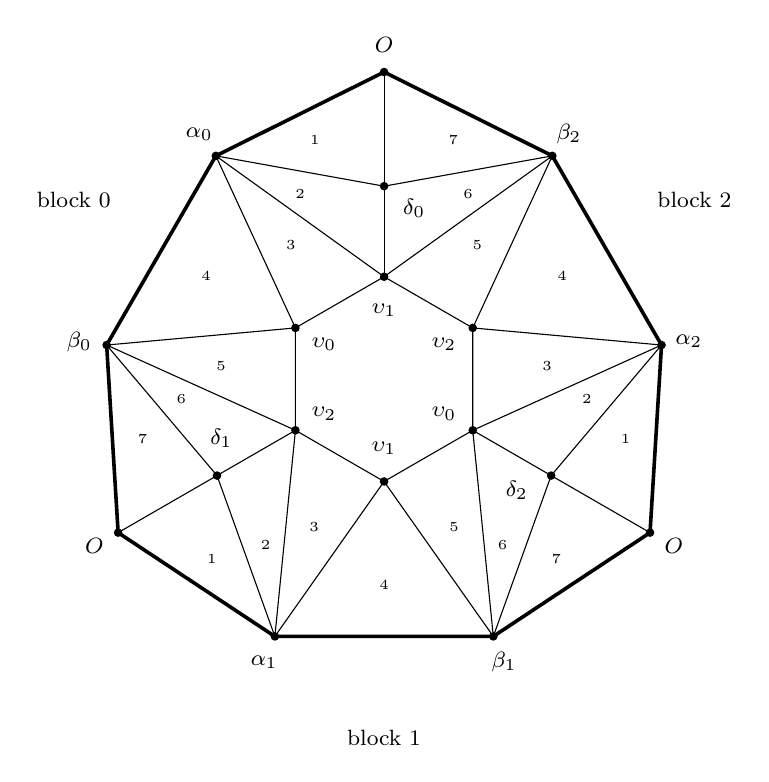
\begin{tikzpicture}[x=1cm,y=1cm,every node/.style={font=\footnotesize},
   dot/.style={circle,fill=black,inner sep=1.1pt},
   lab/.style={fill=white,inner sep=1pt}]
\foreach \i in {0,1,2} {
  \pgfmathsetmacro{\a}{90+120*\i}
  \coordinate (O\i) at (\a:3.9);
  \coordinate (D\i) at (\a:2.45);
  \coordinate (H\i) at (\a:1.3);
  \coordinate (M\i) at (\a+60:1.3);
  \coordinate (A\i) at (\a+37:3.55);
  \coordinate (B\i) at (\a+83:3.55);
}
\foreach \i/\j in {0/1,1/2,2/0} {
  \draw (O\i)--(D\i)--(H\i);
  \draw (D\i)--(A\i)--(H\i)--(M\i)--(A\i);
  \draw (M\i)--(B\i)--(H\j)--(M\i);
  \draw (B\i)--(D\j);
  \draw[line width=1.3pt] (O\i)--(A\i)--(B\i)--(O\j);
  \node at (barycentric cs:O\i=1,D\i=1,A\i=1.4) {\tiny 1};
  \node at (barycentric cs:D\i=1,A\i=2,H\i=1) {\tiny 2};
  \node at (barycentric cs:A\i=1.3,H\i=1,M\i=1) {\tiny 3};
  \node at (barycentric cs:A\i=1,M\i=1,B\i=1) {\tiny 4};
  \node at (barycentric cs:B\i=1.3,M\i=1,H\j=1) {\tiny 5};
  \node at (barycentric cs:B\i=2,H\j=1,D\j=1) {\tiny 6};
  \node at (barycentric cs:B\i=1.4,D\j=1,O\j=1) {\tiny 7};
}
\foreach \i/\j in {0/1,1/2,2/0} {
  \pgfmathsetmacro{\a}{90+120*\i}
  \foreach \p in {O\i,D\i,H\i,M\i,A\i,B\i} \node[dot] at (\p) {};
  \node at (\a:4.25) {$O$};
  \node at (\a+37:3.9) {$\alpha_{\i}$};
  \node at (\a+83:3.9) {$\beta_{\i}$};
  \node[lab] at (\a-10:2.2) {$\delta_{\i}$};
  \node at (\a:0.88) {$\upsilon_{\j}$};
  \node at (\a+60:0.88) {$\upsilon_{\i}$};
  \node at (\a+60:4.55) {block $\i$};
}
\end{tikzpicture}
\caption{The $21$ triangles, drawn as an annulus of three blocks; the numbers $1,\ldots,7$ are those of the triangles within their block. The outer boundary (bold) consists of the three loops $\ell_0,\ell_1,\ell_2$, and its three corners marked $O$ are the same vertex of $\Delta$. The inner hexagon is not a boundary: opposite vertices of the hexagon carry the same label, and opposite edges are the same edge of $\Delta$. Hence every edge that is not bold lies in exactly two of the triangles.}
\label{fig:triangles}
\end{figure}

\emph{The circle space $Z$ and its orbit filling.} The space $Z$ is built from the following pieces.
\begin{itemize}
\item \emph{Six copies of $\mathbb T\times\Delta$,} one for each basis $b\in\{1,\ldots,6\}$. The circle group $\mathbb T$ acts freely on each copy by translation in the first coordinate $t\in\mathbb T$.
\item \emph{Nine cylinders $\mathbb T^2\times[0,1]$,} one for each edge $e=ik$ of $K_{3,3}$ (with $i\le3<k$).
\item \emph{Attachments.} For an end $b\in\{i,k\}$ of $e$, let $r(b,e)\in\mathbb Z/3$ be the index of the loop that corresponds to the plane $P_e$ at basis $b$: if $A_{b,e}$ is $A_q$ or $A_q^c$ with $q\in\{1,2,3\}$, then $r(b,e)=q-1$, which is the index of position $q$ among the tail positions. In particular $r(3,36)=r(6,36)=2$. The point $(t,u,0)$ of the cylinder of $e$ is attached to the point $(t,\ell_{r(i,e)}(u))$ of copy $i$. The point $(t,u,1)$ is attached to the point $(t,\ell_{r(k,e)}(u))$ of copy $k$ if $e\ne36$, and to the point $(t+u,\ell_2(-u))$ of copy $6$ if $e=36$.
\end{itemize}
Thus each cylinder joins the torus $\{(t,\ell_{r(i,e)}(u)):t,u\in\mathbb T\}$ in copy $i$ to the torus $\{(t,\ell_{r(k,e)}(u)):t,u\in\mathbb T\}$ in copy $k$. Every attaching map commutes with translation in $t$. Hence the resulting compact polyhedron $Z$ carries a free $\mathbb T$-action and is a circle space, with half-turn $t\mapsto t+3/2$. Its quotient $Z/\mathbb T$ consists of six copies of $\Delta$ connected along nine cylinders over loops, and it is connected because $\Delta$ is connected.

Write $o\in H_1(Z;\Ftwo)$ for the homology class of a single $\mathbb T$-orbit; because $Z/\mathbb T$ is connected, transporting along a path shows that all orbits represent the same class $o$. For each basis $b\in\{1,\ldots,6\}$ and $m\in\mathbb Z/3$, let $s_{bm}\in H_1(Z;\Ftwo)$ be the class of the loop $u\mapsto(0,\ell_m(u))$ in copy $b$. By the $21$-triangle homology inside $\Delta$,
\[
 \sum_{m\in\mathbb Z/3} s_{bm}=0\qquad\text{for every }b\in\{1,\ldots,6\}.
\]
Across the cylinder of each of the eight uncomplemented edges, the two matched loops $s_{i,r(i,e)}$ and $s_{k,r(k,e)}$ are homotopic and therefore equal in $H_1(Z;\Ftwo)$. Across the cylinder of the complemented edge $36$ of $K_{3,3}$, the loop $u\mapsto(0,\ell_2(u))$ in basis $3$ is homotopic to $u\mapsto(u,\ell_2(-u))$ in basis $6$, whose homology class in the end torus $\mathbb T\times\ell_2(\mathbb T)$ is $o+s_{6,2}$ (both coordinate degrees are odd mod $2$). Thus $s_{3,2}+s_{6,2}=o$. Summing the six chart relations $\sum_m s_{bm}=0$ over all $b=1,\ldots,6$ pairs up all eighteen classes along the nine edges of $K_{3,3}$, yielding $o=0$ in $H_1(Z;\Ftwo)$. Consequently, choosing a point $x_0$ on the orbit of $(0,O)$ in one copy, there exists a singular $2$-chain $x_1\in C_2(Z;\Ftwo)$ with $\partial x_1=Bx_0$.

\emph{Equivariant map $Z\to\B(F_{\rm phys})$.} At any point $(t,p)\in\mathbb T\times\Delta$ in copy $b$, define a pair of probability measures $(\mu_{b,t,p},\nu_{b,t,p})$ on the words of basis $b$ in~\eqref{eq:finite-words} as the laws of the rounded word
\[
 \omega(s,p)=\bigl(\lfloor s\rfloor,\;\lfloor s+p_0\rfloor,\;\lfloor s+p_1\rfloor,\;\lfloor s+p_2\rfloor\bigr)\pmod3
\]
when $s$ is drawn uniformly from $[t,t+1/2]$ (for $\mu_{b,t,p}$) and uniformly from $[t+3/2,t+2]$ (for $\nu_{b,t,p}$), pushing each word forward to its projective measurement in $V(F_{\rm phys})$. Writing $s=\lfloor s\rfloor+\{s\}$, rounding the coordinates of $p+\{s\}\mathbf 1$ always selects a vertex of the minimal ordered simplex of $\mathbb T^3$ containing $p$, which lies in $\Delta$ because $p\in\Delta$; hence $\omega(s,p)$ always belongs to the $39$ retained words~\eqref{eq:finite-words}.

Any word in $\operatorname{supp}\mu_{b,t,p}$ occurs on a set of positive measure in $(t,t+1/2)$, and any word in $\operatorname{supp}\nu_{b,t,p}$ occurs on a set of positive measure in $(t+3/2,t+2)$. For every $s\in(t,t+1/2)$ and $s'\in(t+3/2,t+2)$, the difference $s'-s$ lies strictly in $(1,2)$, so $\lfloor s'+c\rfloor-\lfloor s+c\rfloor\in\{1,2\}$ for every real $c$, hence $\lfloor s+c\rfloor\not\equiv\lfloor s'+c\rfloor\pmod3$. Thus every word in $\operatorname{supp}\mu_{b,t,p}$ differs from every word in $\operatorname{supp}\nu_{b,t,p}$ in all four positions, making their measurements orthogonal at every color and hence adjacent in $F_{\rm phys}$. Writing $s=t+a$ ($a\in[0,1/2]$), the rounding thresholds in $a$ form a finite set of measure zero for every $(t,p)$, so bounded convergence ensures continuity in $(t,p)$. Shifting $t$ by $3/2$ (the half-turn on $Z$) exchanges the intervals $[t,t+1/2]$ and $[t+3/2,t+2]$, hence exchanges the two shores.

Finally, on a matched loop $p=\ell_i(u)=u\alpha_i$, the sampled word $\omega(s,\ell_i(u))$ takes color $\lfloor s\rfloor\pmod3$ on position $0$ and on the tail position indexed by $i$, and color $\lfloor s+u\rfloor\pmod3$ on the other two positions. At every end of a cylinder other than the basis-$6$ end of the complemented edge $36$ of $K_{3,3}$, the former two positions form the set $A_{b,e}$ of plane positions, so the word returns $\lfloor s\rfloor$ on $P_e$ and $\lfloor s+u\rfloor$ on $I-P_e$. At the basis-$6$ end of edge $36$ they form the complement of $A_{6,36}$; there the attaching map replaces $(s,u)$ by $(s+u,-u)$, which turns $(\lfloor s\rfloor,\lfloor s+u\rfloor)$ into $(\lfloor s+u\rfloor,\lfloor s\rfloor)$, so that the word again returns $\lfloor s\rfloor$ on $P_{36}$ and $\lfloor s+u\rfloor$ on $I-P_{36}$. Because the chart maps agree identically on the two ends of every cylinder, extending them constantly along the cylinder parameter $[0,1]$ defines a continuous equivariant map $Z\to\B(F_{\rm phys})$. Together with $(x_0,x_1)$, this forms a tower of length one over $F_{\rm phys}$.
